% METTI SOLO TABELLE E GRAFICI, SU RETROSPETTIVA FAI UNA TABELLA RIASSUNTIVA E COMMENTA I PROBLEMI
\paragraph{MS001 - Numero di metodi}\mbox{}\\[0,3cm]
    \begin{table}[H]
        \centering
        \begin{tabular}{ccccccc}
            \rowcolor{greySWEight}
            \textcolor{white}{\textbf{Codice}} &
            \textcolor{white}{\textbf{File analizzati}}&
            \textcolor{white}{\textbf{Media metodi per classe}}&
            \textcolor{white}{\textbf{Riscontro}}\\
            \textbf{MS001} & 44 & 2.47 & \textcolor{ForestGreen}{Ottimale}\\
        \end{tabular}
        \caption{Media metodi per classe}
    \end{table}

    \begin{figure}[H]
        \centering
        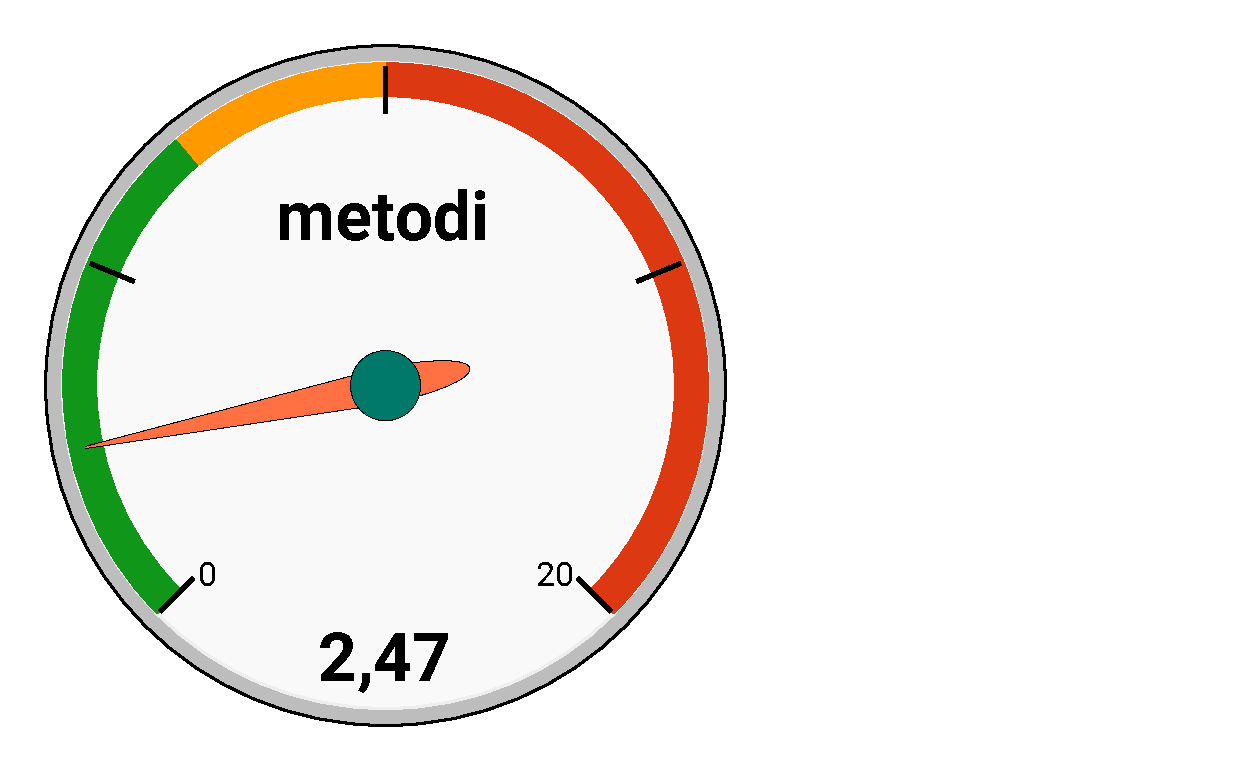
\includegraphics[width=50mm]{sez/App_Esito/Qualifica/graph/numeroMetodiCruscotto.pdf}
        \caption{Media metodi per classe nel periodo di Codifica}
    \end{figure}

\paragraph{MS002 - Numero di parametri}\mbox{}\\[0,3cm]
    \begin{table}[H]
        \centering
        \begin{tabular}{ccccc}
            \rowcolor{greySWEight}
            \textcolor{white}{\textbf{Codice}} &
            \textcolor{white}{\textbf{File analizzati}} &
            \textcolor{white}{\textbf{[5,8] parametri}}&
            \textcolor{white}{\textbf{8 o più parametri}}&
            \textcolor{white}{\textbf{Riscontro}}\\
            \textbf{MS001} & 44 & 2 & 0 & \textcolor{YellowOrange}{Accettabile}\\
        \end{tabular}
        \caption{Media parametri dei metodi nel periodo di Codifica}
    \end{table}
    \begin{figure}[H]
        \centering
        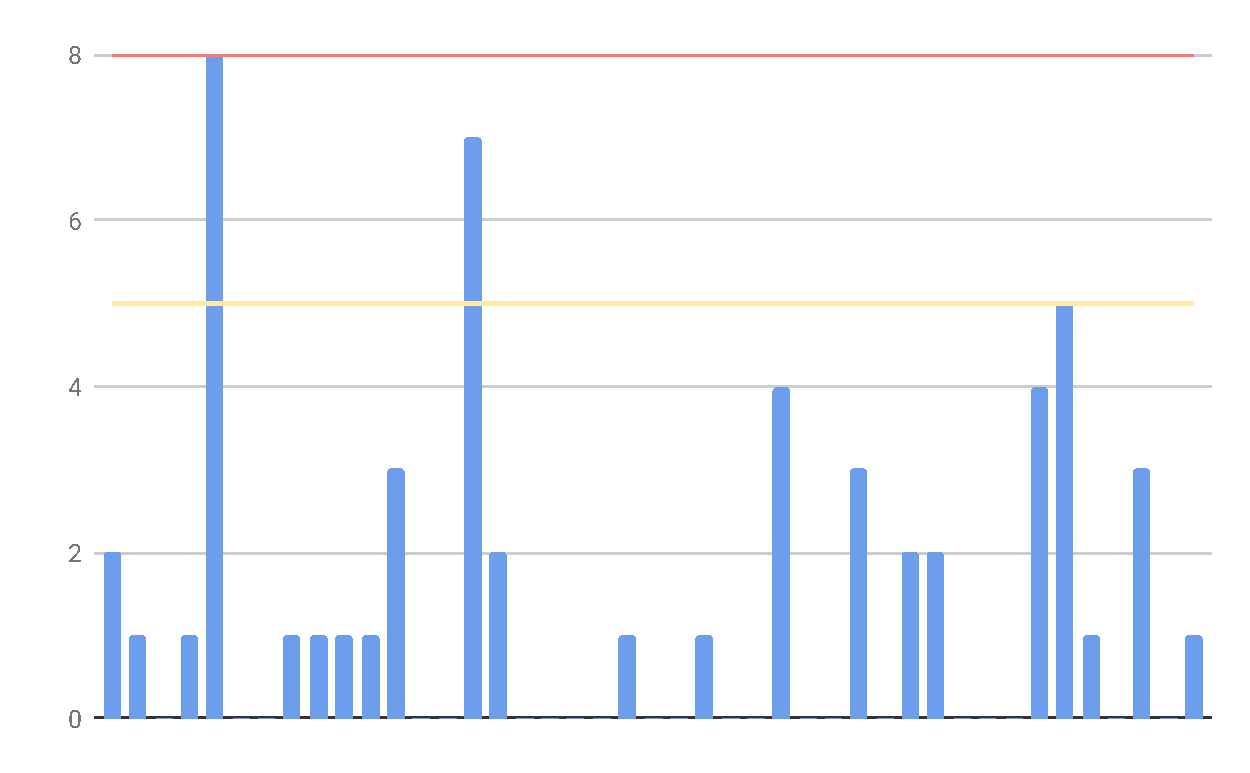
\includegraphics[width=0.7\linewidth]{sez/App_Esito/Qualifica/graph/parametriPerMetodo.pdf}
        \caption{Parametri dei metodi nel periodo di Codifica}
    \end{figure}
    \begin{figure}[H]
        \centering
        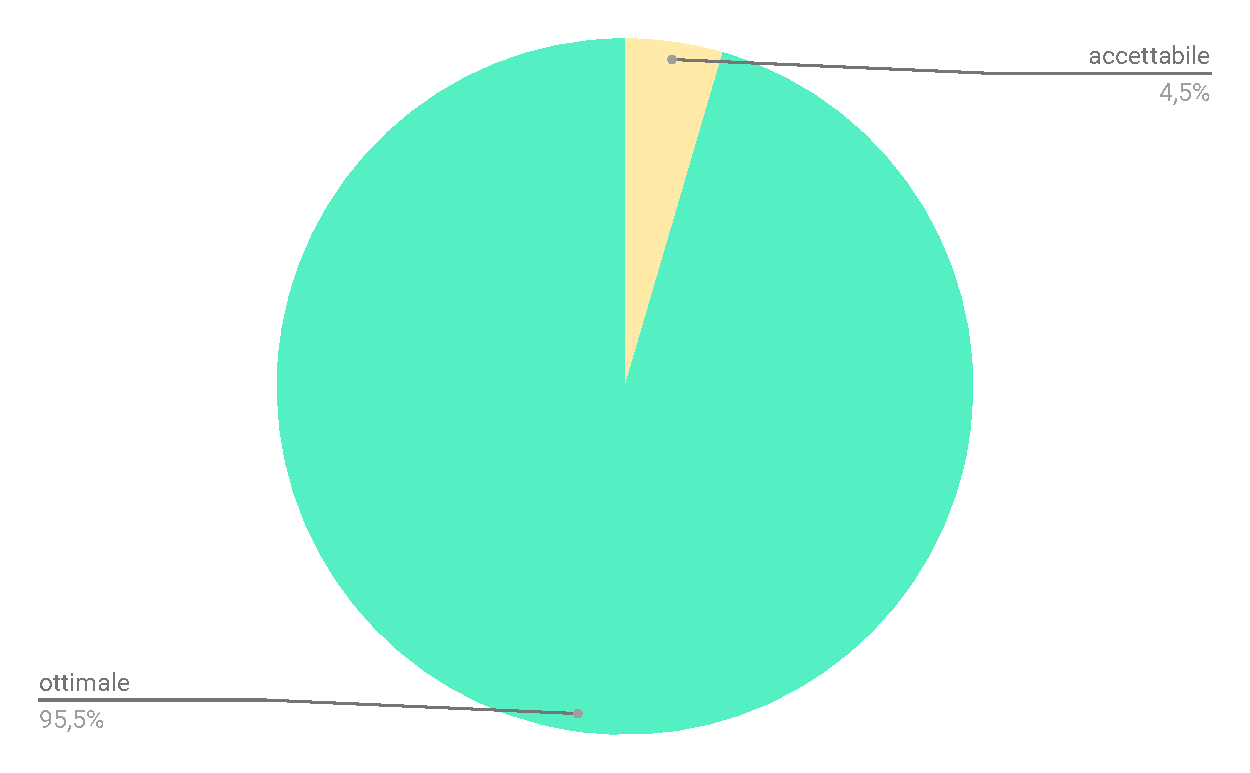
\includegraphics[width=0.7\linewidth]{sez/App_Esito/Qualifica/graph/parametriPerMetodoTorta.pdf}
        \caption{Percentuale test dei parametri superati nel periodo di Codifica}
    \end{figure}

\paragraph{MS003 - Funzioni di interfaccia per package}\mbox{}\\[0,3cm]
    \begin{table}[H]
        \centering
        \begin{tabular}{ccccc}
            \rowcolor{greySWEight}
            \textcolor{white}{\textbf{Codice}} &
            \textcolor{white}{\textbf{File analizzati}} &
            \textcolor{white}{\textbf{Valore}}&
            \textcolor{white}{\textbf{Riscontro}}\\
            \textbf{MS003} & 44 & 1.23 & \textcolor{ForestGreen}{Ottimale}\\
        \end{tabular}
        \caption{Media metodi per classe}
    \end{table}
    \begin{figure}[H]
        \centering
        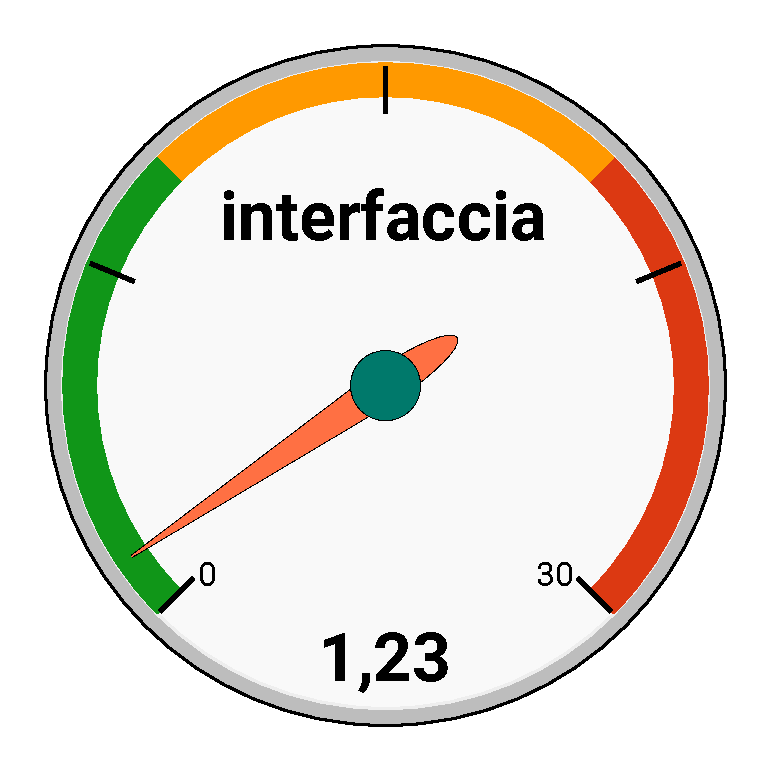
\includegraphics[width=50mm]{sez/App_Esito/Qualifica/graph/interfacciaPerP.pdf}
        \caption{Interfacce}
    \end{figure}

\paragraph{MS004 - Complessità ciclomatica}\mbox{}\\[0,3cm]
    \begin{table}[H]
        \centering
        \begin{tabular}{ccccccc}
            \rowcolor{greySWEight}
            \textcolor{white}{\textbf{Codice}} &
            \textcolor{white}{\textbf{File analizzati}} &
            \textcolor{white}{\textbf{Valore}}&
            \textcolor{white}{\textbf{Riscontro}}\\
            \textbf{MS004} & 44 & 1.54 & \textcolor{ForestGreen}{Ottimale}\\
        \end{tabular}
        \caption{Campi dati per classe nel periodo di Codifica}
    \end{table}
    \begin{figure}[H]
        \centering
        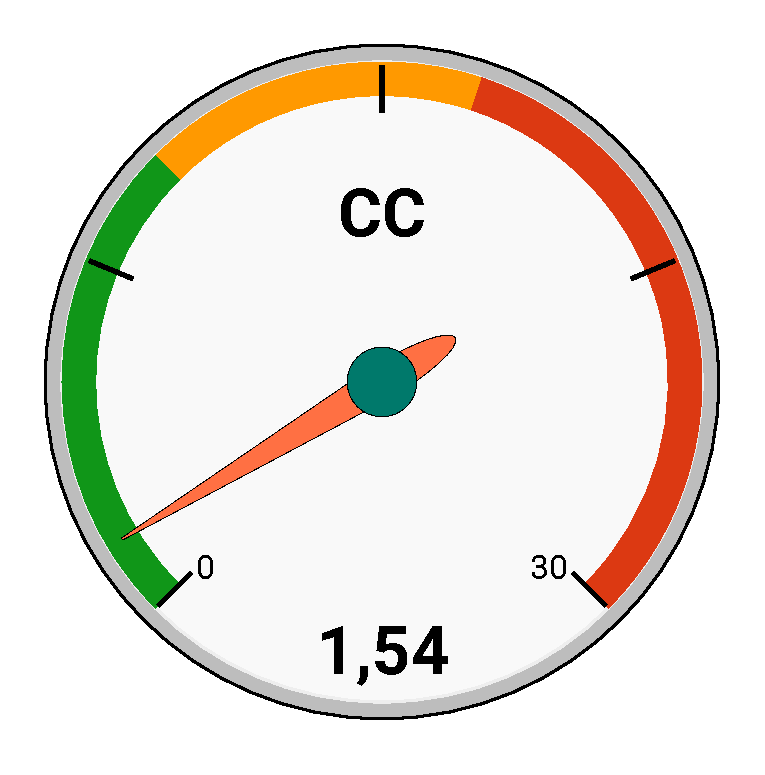
\includegraphics[width=50mm]{sez/App_Esito/Qualifica/graph/complCCruscotto.pdf}
        \caption{Complessità ciclomatica periodo di codifica}
    \end{figure}

\paragraph{MS005 - Campi dati per classe}\mbox{}\\[0,3cm]
    \begin{table}[H]
        \centering
        \begin{tabular}{ccccccc}
            \rowcolor{greySWEight}
            \textcolor{white}{\textbf{Codice}} &
            \textcolor{white}{\textbf{File analizzati}}&
            \textcolor{white}{\textbf{Riscontro}}\\
            \textbf{MS005} & 44 & \textcolor{YellowOrange}{Accettabile}\\
        \end{tabular}
        \caption{Campi dati per classe nel periodo di Codifica}
    \end{table}
    \begin{figure}[H]
        \centering
        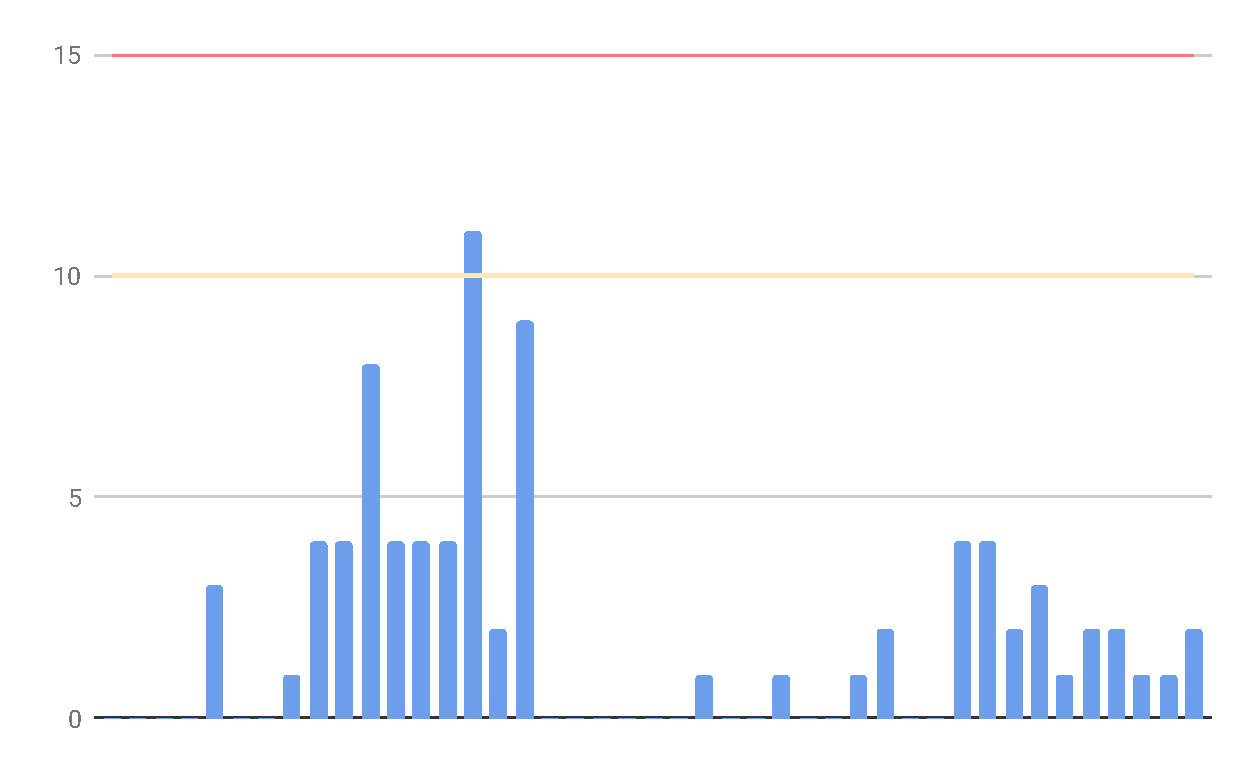
\includegraphics[width=0.7\linewidth]{sez/App_Esito/Qualifica/graph/campiDatiPerClasse.pdf}
        \caption{Numero di campi dati per classe nel periodo di Codifica}
    \end{figure}
    \begin{figure}[H]
        \centering
        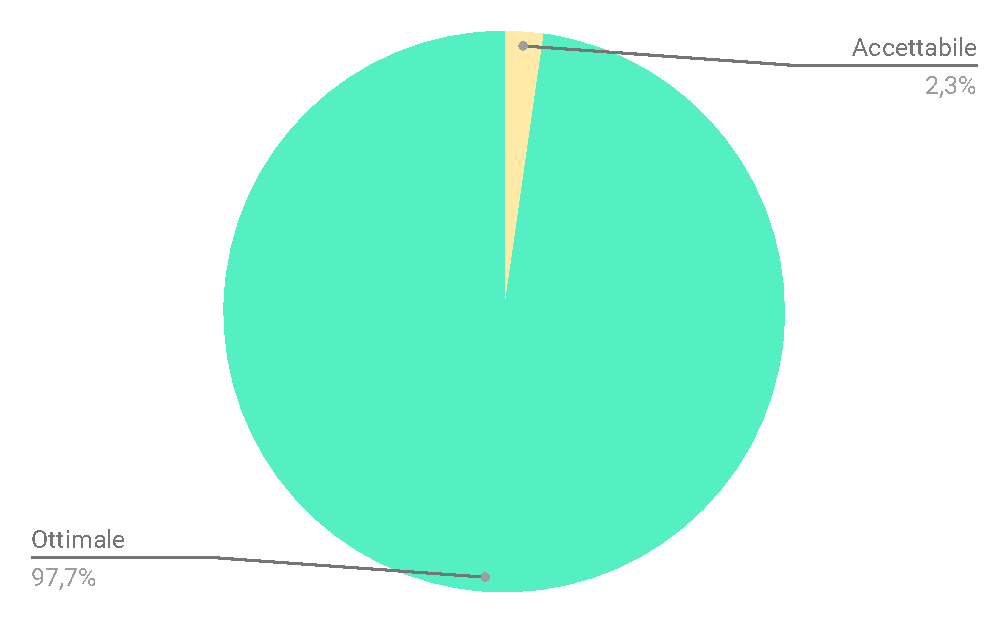
\includegraphics[width=0.7\linewidth]{sez/App_Esito/Qualifica/graph/campiDatiPerClasseTorta.pdf}
        \caption{Percentuale test dei campi dati superati nel periodo di Codifica}
    \end{figure}

\paragraph{MS006 - Commenti per linee di codice}\mbox{}\\[0,3cm]
    \begin{table}[H]
        \centering
        \begin{tabular}{ccccccc}
            \rowcolor{greySWEight}
            \textcolor{white}{\textbf{Codice}} &
            \textcolor{white}{\textbf{File analizzati}}&
            \textcolor{white}{\textbf{Totale righe}}&
            \textcolor{white}{\textbf{Totale righe commento}}&
            \textcolor{white}{\textbf{Percentuale}}&
            \textcolor{white}{\textbf{Riscontro}}\\
            \textbf{MS006} & 92 & 7524 & 945 & 12.56\% & \textcolor{YellowOrange}{Accettabile}\\
        \end{tabular}
        \caption{Totale commenti per linee di codice nel periodo di Codifica}
    \end{table}
    \begin{figure}[H]
        \centering
        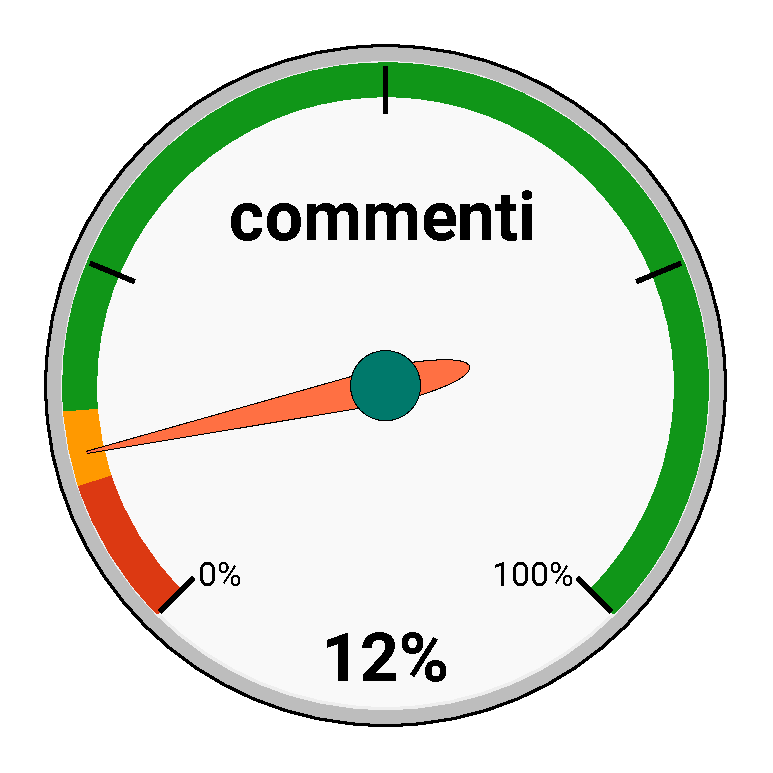
\includegraphics[width=0.3\linewidth]{sez/App_Esito/Qualifica/graph/commenti.pdf}
        \caption{Percentuale commenti per linee di codice periodo di codifica}
    \end{figure}

\paragraph{MS007 - Code coverage}\mbox{}\\[0,3cm]
    \begin{table}[H]
        \centering
        \begin{tabular}{ccccc}
            \rowcolor{greySWEight}
            \textcolor{white}{\textbf{Codice}} &
            \textcolor{white}{\textbf{Valore}}&
            \textcolor{white}{\textbf{Riscontro}}\\
            \textbf{MS007} & 85.18\% & \textcolor{YellowOrange}{Accettabile}\\
        \end{tabular}
        \caption{Code coverage nel periodo di Codifica}
    \end{table}
    \begin{figure}[H]
        \centering
        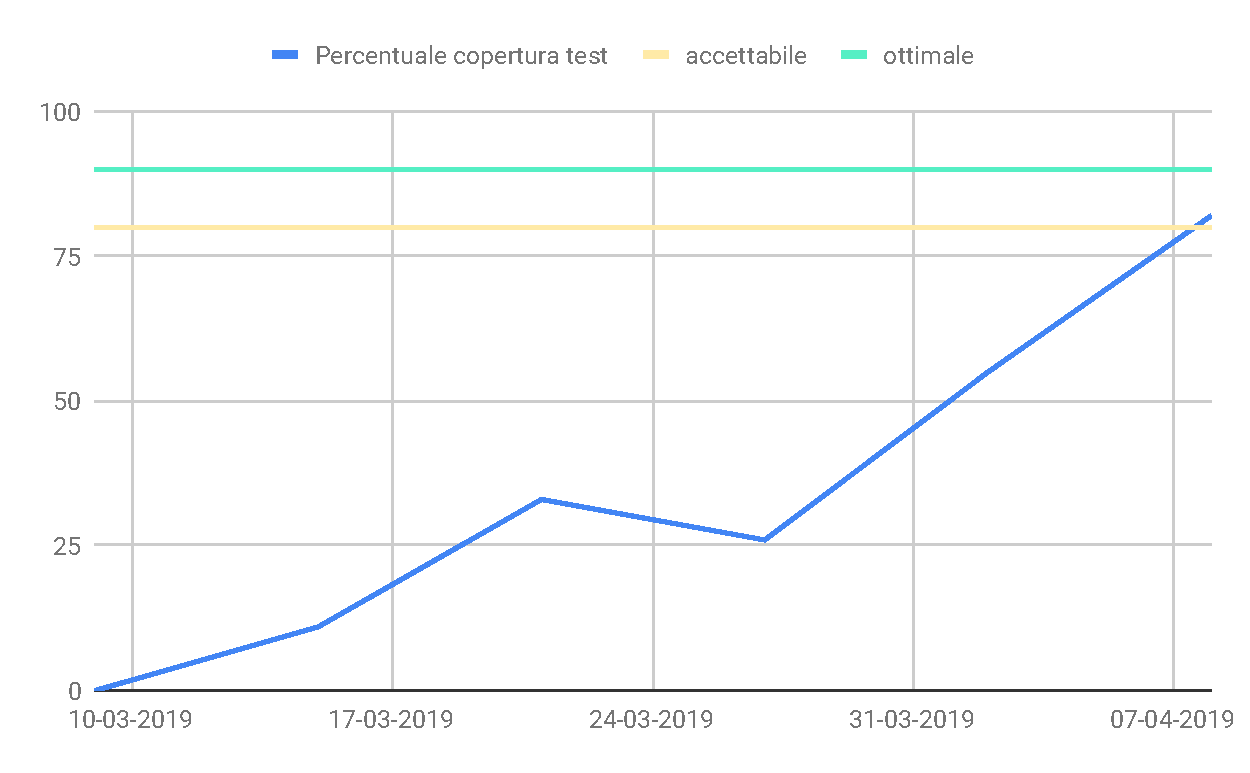
\includegraphics[width=0.7\linewidth]{sez/App_Esito/Qualifica/graph/storicoCodeCoverage.pdf}
        \caption{Storico Code Coverage periodo di Codifica}
    \end{figure}

\paragraph{MS008 - Superamento test}\mbox{}\\[0,3cm]
    \begin{table}[H]
        \centering
        \begin{tabular}{cccc}
        \rowcolor{greySWEight}
        \textcolor{white}{\textbf{Codice}} &
        \textcolor{white}{\textbf{Nome}} &
        \textcolor{white}{\textbf{Valore}} &
        \textcolor{white}{\textbf{Riscontro}}\\
        \textbf{MS008}& Test superati & 100\% & \textcolor{ForestGreen}{Ottimale} \\

        \end{tabular}
        \caption{Percentuale di test superati nel periodo di codifica}
    \end{table}

\paragraph{MS009 - Soddisfacimento requisiti obbligatori}\mbox{}\\[0,3cm]
    \begin{table}[H]
        \centering
        \begin{tabular}{cccc}
        \rowcolor{greySWEight}
        \textcolor{white}{\textbf{Codice}} &
        \textcolor{white}{\textbf{Requisiti obbligatori soddisfatti}} &
        \textcolor{white}{\textbf{Riscontro}}\\
        \textbf{MS009}& 77.40\% & \textcolor{BrickRed}{Non accettabile} \\

        \end{tabular}
        \caption{Requisit obbligatori soddisfatti nel periodo di codifica}
    \end{table}
    \begin{figure}[H]
        \centering
        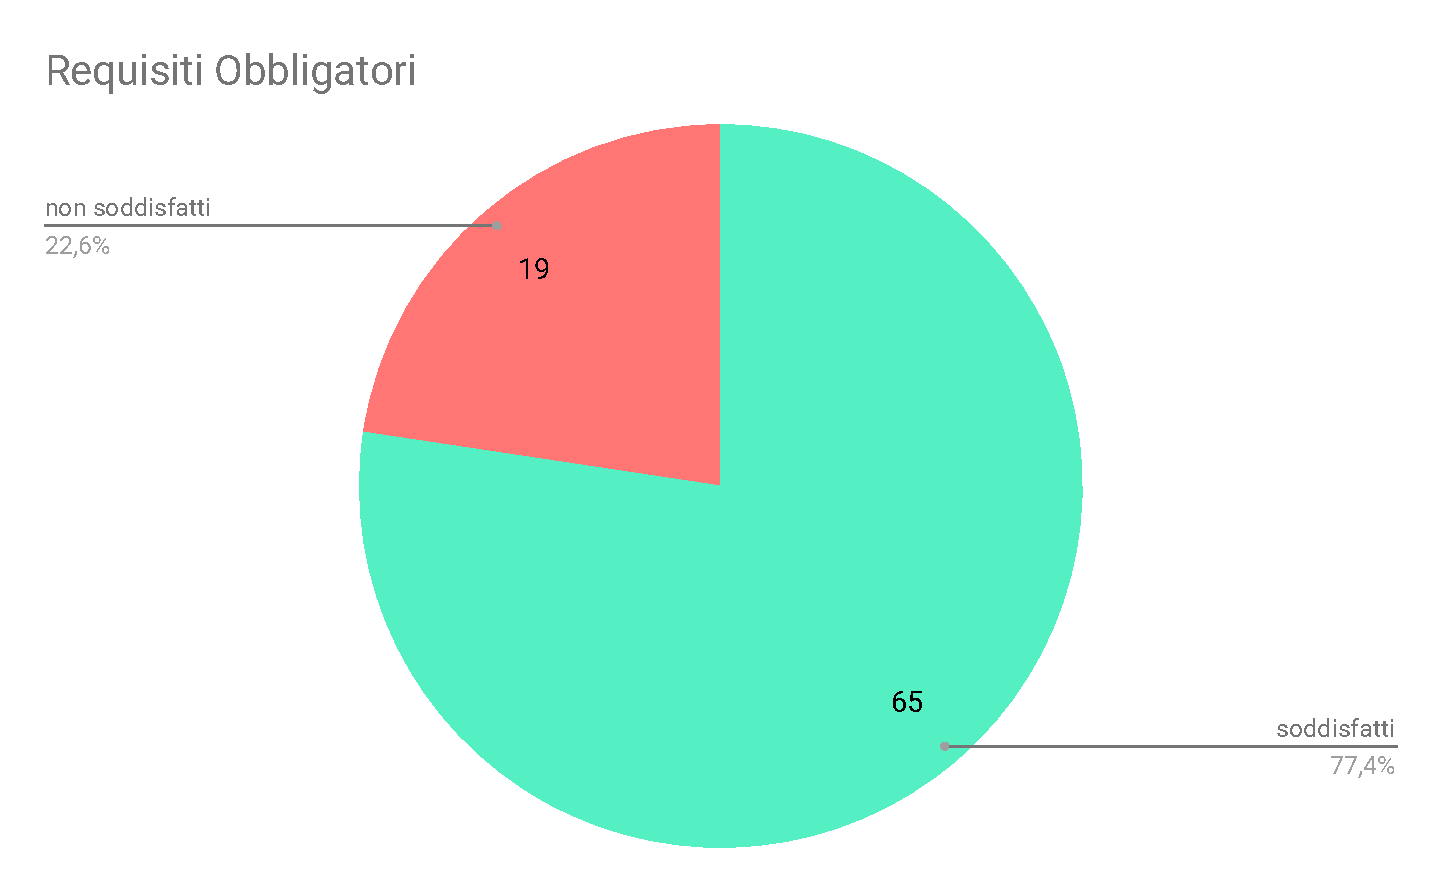
\includegraphics[width=0.7\linewidth]{sez/App_Esito/Qualifica/graph/RequisitiObbligatori.pdf}
        \caption{Soddisfacimento requisiti obbligatori nel periodo di Codifica}
    \end{figure}

\paragraph{MS010 - Media di build Travis settimanali}\mbox{}\\[0,3cm]
    Estrapolando i dati dagli insights del sito di Travis è stata riscontrata una media di build settimanali di 70.75.

    \begin{table}[H]
        \centering
        \begin{tabular}{cccc}
        \rowcolor{greySWEight}
        \textcolor{white}{\textbf{Codice}} &
        \textcolor{white}{\textbf{Media}} &
        \textcolor{white}{\textbf{Riscontro}}\\
        \textbf{MS010}& 70.75 & \textcolor{ForestGreen}{Ottimale} \\
    
        \end{tabular}
        \caption{Media build settimanali nel periodo Codifica}
    \end{table}
    \begin{figure}[H]
        \centering
        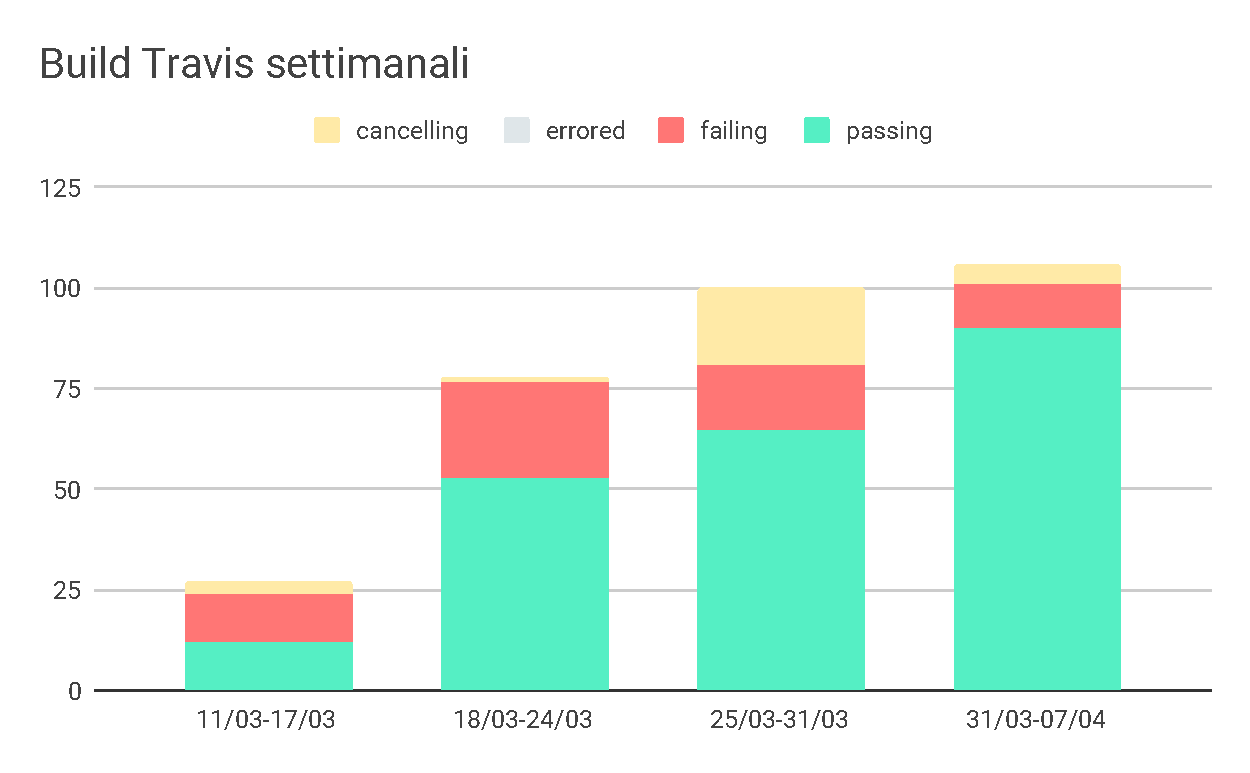
\includegraphics[width=0.7\linewidth]{sez/App_Esito/Qualifica/graph/buildTravisSettimanale.pdf}
        \caption{Build di Travis settimanali, dal 2019-03-11 al 2019-04-07}
    \end{figure}

    \paragraph{MS011 - Percentuale build Travis superate }\mbox{}\\[0,3cm]
    
    \begin{table}[H]
        \centering
        \begin{tabular}{c c c c c}
        \rowcolor{greySWEight}
        \textcolor{white}{\textbf{Codice}} &
        \textcolor{white}{\textbf{Range accettabile}} &
        \textcolor{white}{\textbf{Range ottimale}} &
        \textcolor{white}{\textbf{build superate}} &
        \textcolor{white}{\textbf{Riscontro}}\\
        \textbf{MS011} & $[75\%,100\%]$ & $[85\%,100\%]$ & 71.40\% & \textcolor{RubineRed}{non superato} \\
    
        \end{tabular}
        \caption{Build Travis superate nel periodo di Codifica}
    \end{table}
    \begin{figure}[H]
        \centering
        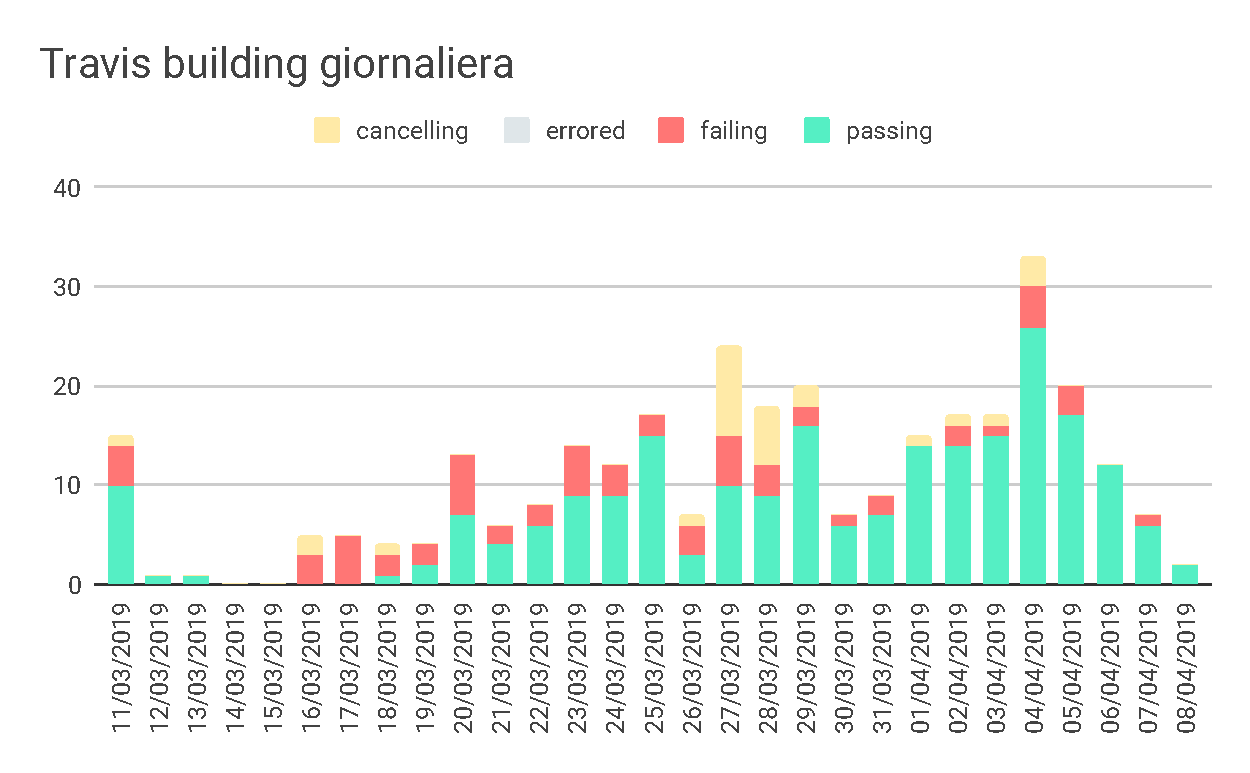
\includegraphics[width=0.7\linewidth]{sez/App_Esito/Qualifica/graph/buildTravisGiornaliera.pdf}
        \caption{Build di Travis giornaliere, dal 2019-03-11 al 2019-04-07}
    \end{figure}
    \begin{figure}[H]
        \centering
        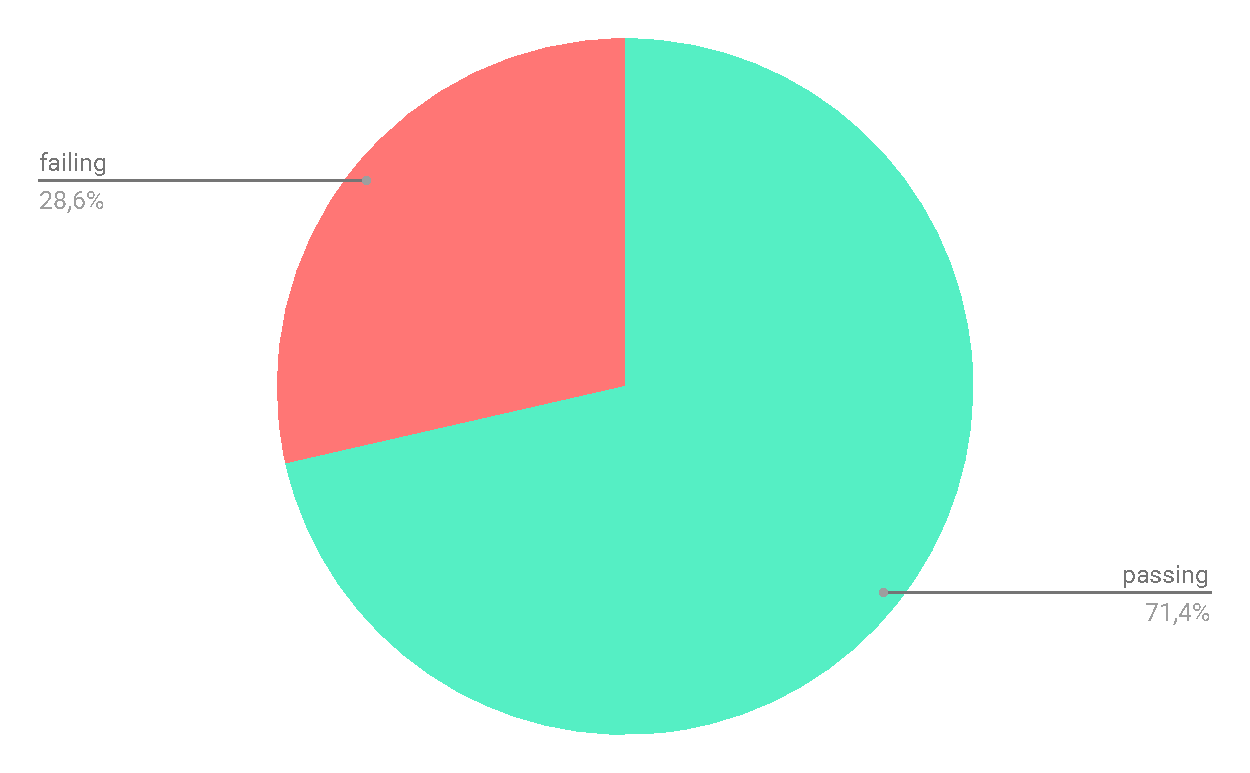
\includegraphics[width=0.7\linewidth]{sez/App_Esito/Qualifica/graph/buildTravisSuperate.pdf}
        \caption{Build di Travis superate nel periodo di Codifica}
    \end{figure}